\newpage
\section{Ambient Air Pollution \& Electricity Generation}

The previous two chapters have focused on preparing a broad base of knowledge on climate economics---the first chapter by reviewing the physical science of climate change and the second chapter by reviewing the economics of climate policy design. This chapter continues to build background, but focuses instead on providing context specific to the modeling and empirical work done in the two chapters that follow it. 

To motivate these proceeding chapters, this chapter begins by discussing ambient air pollution with particular emphasis on the impacts of ambient air pollution and air pollution disparities. As alluded to earlier, the ultimate goal is to model and simulate these air pollution disparities that result from the implementation of a carbon tax on the electric power industry in California. Keeping this in mind, the discussion on air pollution is followed by an overview of wholesale electricity markets and Assembly Bill 32 (AB-32), the California statute that creates an emissions trading program across the state. Finally, I review the body of literature immediately adjacent to this research. The related literature serves both to establish what we already know about the implications of carbon pricing for environmental inequality and to motivate the specific goals of the research in this paper. This chapter concludes by describing the overall research design that unfolds in the next two chapters. The description of this design is outlines both the research design choices I make in these later chapters and the motivation for these design choices. 

\subsection{Primer on Ambient Air Pollution}

\noindent Introduction
\begin{itemize}
    \item What is ambient air pollution? 
    \item What are the most common air pollutants?
\end{itemize}

Ambient air pollution exposure comes with many negative consequences, but the most striking of these is the effect of ambient air pollution on human health and mortality. \textbf{Talk about the mechanisms using \cite{aguilar2022air}}.

The World Health Organization (WHO) estimates that ambient air pollution caused over 4.2 million premature deaths in 2019, making ambient air pollution one of the leading global health stressors \citep{who_factsheet}. Around the world, 99\% of people live in environments that do not meet the WHO's air quality guidelines. Understandably, the vast majority (89\%) of these premature deaths are in low- and middle-income countries, but ambient air pollution remains a serious health threat even in wealthy nations, including the US. \cite{lelieveld2019effects} uses atmospheric models alongside a global exposure mortality model---a model that maps air pollutant concentrations into mortalities---to study excess mortalities attributable to anthropogenic air pollution emissions. They find that ambient air pollutants from anthropogenic sources (primarily the burning od fossil fuels) result in 230,000 excess deaths annually in the US.\footnote{
    The 95\% confidence interval around these estimates is 184,000--276,000 excess deaths---a wide interval, but an interval where even the minimum of the interval warrants serious concern.
} 

Apart from the devastating effects of air pollution on human health, the other primary effect of air pollution exposure is reduced cognitive performance and decision making. \cite{fonken2011air} find physical changes in the brains of mice who have been exposed to fine particulate matter at concentrations and durations comparable to Beijing. Namely, they find that neurons in the hippocampus---an area of the brain devoted to memory and learning---have shorter and less dense dendrites. These dendrites are responsible for receiving signals from other neurons, and the reduced length and density of these neurons is correlated with poorer memory \citep{weir2012smog}.Additionally, the mice exposed to particulate matter display depressive-like symptoms, giving up earlier in forced swimming tests and eating less. 

These physiological findings in mice correspond with a wealth of evidence on the effects of air pollution on human learning and cognition. \cite{aguilar2022air} provides the best review of these effects and their implications for human capital formation and labor economics more broadly. 

\noindent Education/Human Capital Development \& Labor Implications
\begin{itemize}
    \item \cite{zhang2018impact}
    \item \cite{currie2014we}
    \item \cite{aguilar2022air}
    \item \cite{currie2009does}
    \item \cite{ebenstein2016long}
    \item \cite{chang2016particulate}
\end{itemize}




\noindent Crime
\begin{itemize}
    \item \cite{bondy2020crime}
    \item \cite{burkhardt2019effect}
\end{itemize}

\noindent Happiness
\begin{itemize}
    \item \cite{zheng2019air}
\end{itemize}

Together, the many effects of air pollution add to the popular 






\noindent Justice/Inequality/Distributional perspectives
\begin{itemize}
    \item \cite{colmer2020disparities}
    \item \cite{hernandez2022decomposing}
    \item \cite{currie2023caused}
    \item \cite{banzhaf2019environmental}
    \item \cite{voorheis2017air}
\end{itemize}






\subsection{The Case of California: Electricity \& AB-32}

\begin{figure}
    \centering
    \caption{Western Interconnection Subregions}
    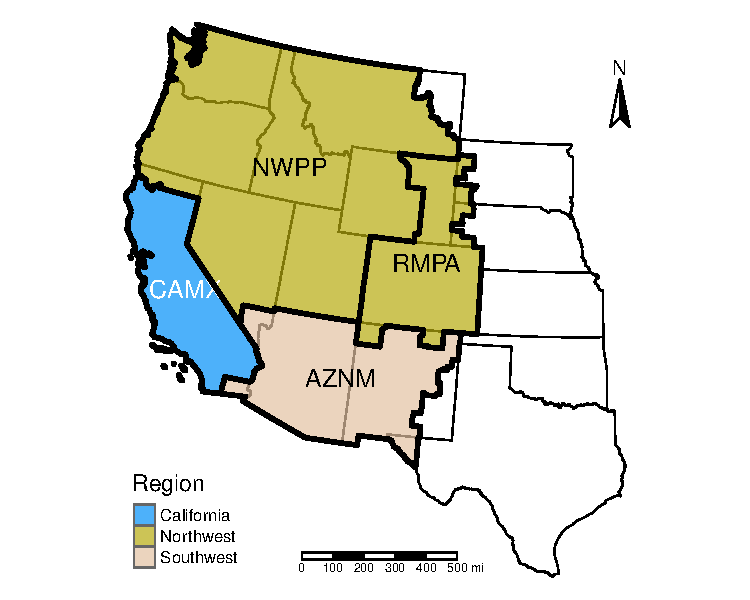
\includegraphics[width=0.8\textwidth]{figures/chapter3_figures/WECC_map.pdf}
    \fignote[1]{Figure displays the subregions of the Western Interconnection. These subregions are a unit of geography set by the North American Electric Reliability Council (NERC). NERC determines these regions based off of the connections/boundaries between balancing authorities, the administrative unit of the US power grid. These regions are the California-Mexico Power Area (CAMX), the Northwest Power Pool Area (NWPP), the Rocky Mountain Power Area (RMPA), and the Arizona-New Mexico-Southern Nevada Power Area (AZNM). The EPA reports data for each of the four NERC regions, but the EIA only provides electricity demand data for the NWPP and RMPA together. These two subregions are treated as one throughout the paper, and future chapters will model just the three regional markets displayed: the California market, the Southwest market, and the Northwest market. Shapefiles for the regions come from \cite{HIFLD_nerc}.
    }
\end{figure}

\begin{figure}
    \centering
    \caption{California Emissions Allowance Price}
    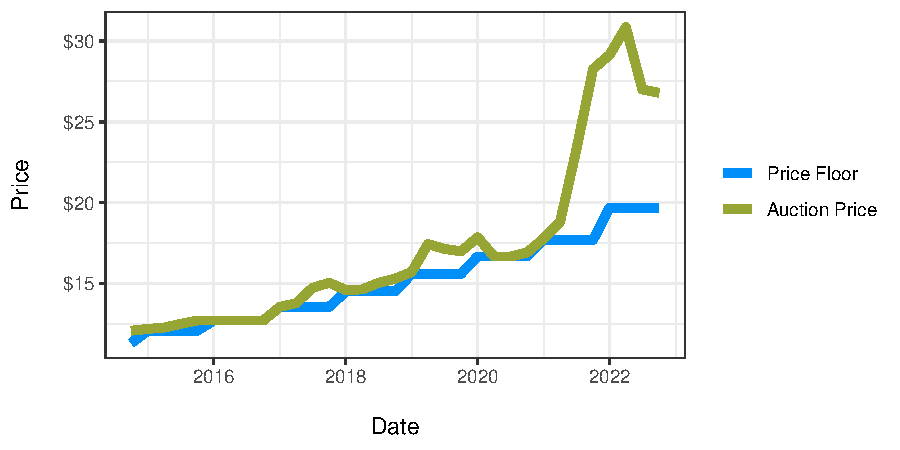
\includegraphics[width=\textwidth]{figures/chapter3_figures/allowance_prices.pdf}
    \fignote[1]{Figure displays the auction price and price floor for emissions allowances in California from Q4 2015 through Q4 2022. Each emissions allowance covers one tonne of CO$_2$e emissions. Data on emissions allowances come from the California Air Resources Board, \cite{carb_prices}.}
\end{figure}


\noindent Wholesale electricity markets: How they work and their ``competitiveness"
\begin{itemize}
    \item \cite{ferc2020}
\end{itemize}

\noindent Short history of CAISO
\begin{itemize}
    \item \cite{sweeney2013california}
    \item \cite{knittel2005empirical}
    \item \cite{borenstein2000diagnosing}
    \item \cite{borenstein2015us}
\end{itemize}

\noindent Leakage
\begin{itemize}
    \item \cite{burtraw2018}
    \item \cite{fowlie2009incomplete}
    \item \cite{fowlie2021border}
\end{itemize}

\noindent Effect of AB-32 on Electricity
\begin{itemize}
    \item \url{https://ww2.arb.ca.gov/our-work/programs/cap-and-trade-program/cap-and-trade-
    regulation}
\end{itemize}

\subsection{Carbon Pricing \& Environmental Inequality}

Carbon pricing policies are highly popular among economists. In what is likely the greatest display of consensus on climate policy from the economics discipline, most all of the nation's leading economists endorsed a series of policy recommendations published in the Wall Street Journal in 2019. The statement titled ``Economists' Statement on Carbon Dividends" calls for the implementation of a nationwide tax on greenhouse gas emissions, border carbon adjustments, and carbon dividends to redistribute the collected tax revenue. Original signatories of the statement include twenty-eight Nobel Laureates, four former Chairs of the Federal Reserve, and fifteen former Chairs of the Council of Economic Advisors. Since its initial release, the statement has earned the signature of thousands of other economists.\footnote{This includes many other well-known economists, like Susan Athey, Daron Acemoglu, and Rick Eichhorn.}

As discussed in Chapter 2, the primary appeal of carbon pricing for economists is the cost-minimizing nature of these policies. The consensus statement's first policy recommendation states this unambiguously:
\begin{quote}
    ``A carbon tax offers the most cost-effective lever to reduce carbon emissions at the scale and speed that is necessary. By correcting a well-known market failure, a carbon tax will send a powerful price signal that harnesses the invisible hand of the marketplace to steer economic actors towards a low-carbon future." 
\end{quote}




It is also relevant to note that the signing economists address how the revenue generated from the carbon price should be distributed---an aspect that if done poorly could create major inequality concerns. The statement's fifth and final policy recommendation reads: 
\begin{quote}
    ``To maximize the fairness and political viability of a rising carbon tax, all the revenue should be returned directly to U.S. citizens through equal lump-sum rebates. The majority of American families, including the most vulnerable, will benefit financially by receiving more in `carbon dividends' than they pay in increased energy prices."
\end{quote}
Together the policy recommendations in the statement provide a brief but clear strategy for reducing greenhouse gas emissions in a manner that is both efficient and progressive in the sense that tax revenue would flow towards those at the bottom end of the income distribution. 

Despite the carbon-pricing fervor of economists, many in the climate policy community remain skepitcal of proposals that rely heavily on carbon pricing for decarbonization. There are a number of arguments against carbon pricing that critique the efficacy of these programs relative to their alternatives, but these concerns are not new and generally struggle to make a strong case.\footnote{Chapter 2 describes arguments against carbon pricing that critique the efficacy of these programs. This discussion comes to four primary conclusions. First, there is a need for additional research that measures the ex-post effect of carbon pricing on emissions reductions. Second, many jurisdictions with carbon pricing programs have chosen to rely on other regulations to attain emissions targets. That is, the implicit price on emissions from other regulations is often higher than the market price of emissions, which can make the effect of emissions pricing appear weak relative to other regulations. Third, in situations where policymakers rely primarily on carbon pricing more so than other regulations, carbon pricing does appear to be the more cost-effective policy. This difference appears to be small though, especially in the electricity market where the strong correlation between the merit order of generation and emissions intensity mean that clean energy standards perform only negligibly worse carbon pricing. Fourth, there are likely tangible improvements to emissions trading programs that can be made, such as reforming or eliminating the use of emissions offsets. 
} Instead, more recent criticism of these policies has centered around their potential to perpetuate environmental inequality. Because global air pollutants (i.e., greenhouse gases) are often released at the same time as local air pollutants (i.e., criteria air pollutants, including PM, NO$_x$, SO$_2$), carbon pricing has the potential to shift the distribution of ambient air pollution. In this context, the less-regulated local air pollutants are often called copollutants. The concern is that even if environmental markets can induce abatement efficiently, the ``invisible hand'' economists celebrate might just shift the burden of air pollution towards already disadvantaged communities. Raising this possibility is entirely fair. After all, the decentralized nature of market means there is no specific mechanism to prevent this from happening. The most vulnerable in society may already feel disenfranchised by market-systems, so the resistance to a cap-and-trade program---a market-based policy instrument---is not entirely surprising. 

Many Californians have expressed concerns about the potential for California's cap-and-trade program to redistribute the air pollution burden towards communities with already poor environmental quality and economic status. In fact, the first question on the ``Frequently Asked Questions'' page of California's cap-and-trade program's website reads: ``Does the cap-and-trade program lead to increases of air pollution in environmental justice communities burdened with air pollution?'' \citep{carb_FAQ}. This was not a major concern when AB-32 was originally passed in 2006, but nearly ended California's cap-and-trade program when it needed to be reauthorized ten years later in 2016 \citep{johnson2020cap}. 

% \citep{johnson2020cap} recounts the political drama surrounding the 2016 reauthorization of California's cap-and-trade program, where many environmental justice advocates pushed for more localized controls air pollutants

% It is important to be clear about the tradeoff this analysis looks at. 

% There is a separate political tradeoff 
% \begin{quote}
%     Most environmental justice advocates aren't fundamentally opposed to putting a price on carbon; they are opposed to the political pattern, repeated several times over, where politicians trade away working local air pollution laws to tackle the global problem of climate change.
% \end{quote}

% The goal of this analysis is not to , 

% Economists \emph{love} carbon pricing, others are less keen (distributional reasons)
% \begin{itemize}
%     \item \cite{fischer2021green}
%     \item \cite{borenstein2022carbon}
% \end{itemize}

% \begin{itemize}
%     \item \url{https://grist.org/climate/the-biggest-fight-over-cap-and-trade-isnt-about-what-you-think-it-is/}
%     \item \url{https://ww2.arb.ca.gov/resources/documents/faq-cap-and-trade-program}
% \end{itemize}

These concerns were intensified following the release of several descriptive analyses that seemed to indicate that California's cap-and-trade program had done exactly that: redistributed air pollution towards disadvantaged communities. \cite{cushing2018carbon}, circulated at the time as \cite{cushing2016preliminary}, notes that even though total emissions from regulated facilities decreased in the three years after the implementation of California's cap-and-trade program, 52\% of facilities actually increased their emissions. Further, \cite{cushing2018carbon} finds that the communities with increases in co-pollutant emissions are on average poorer, less educated, and have a higher proportion of non-white residents than communities with decreases in co-pollutant emissions. In a follow-up study with a few additional years worth of data, \cite{pastor2022up} found similar results. The median facility covered by the cap-and-trade program in a disadvantaged community increased its PM10 emissions by 3.1\%, while the median facility covered by the cap-and-trade program in a non-disadvantaged community decreased its PM10 emissions by 6.9\%---a 10 percentage point difference in changes of PM10 emissions. Other air pollutants show similar disparities in pollution changes, though these differences are only statistically significant at the 5\% level for PM10 and SO$_x$, not for PM2.5, NO$_x$, or greenhouse gas emissions themselves. 

While these two studies help establish important descriptions of environmental justice outcomes in California, as \cite{hernandez2022importance} note, these do little to speak to the actual effect of the cap-and-trade program. First, their results cannot disentangle the effects of the cap-and-trade program from contemporaneous events that may cause the redistribution of co-pollutants. Pollution intensive activities are highly responsive to macroeconomic trends, and it is entirely possible that the redistribution of co-pollutants towards disadvantaged communities is a consequence of these macroeconomic trends rather than the effects of the cap-and-trade program. Second, co-pollutants are often not stagnant, but move into neighboring communities based on geography and atmospheric conditions. This means that even if the emissions of co-pollutants increases in a community, this is not sufficient information to suggest that the air pollution exposure in that community increases as well. 

\cite{hernandez2023environmental} is the first study to provide credible causal measurements of the impact of the cap-and-trade program on air pollution exposure. The authors define and measure changes in the ``environmental justice gap,'' the average difference in air pollution concentrations between disadvantaged and other communities.\footnote{California designates certain census tracts as ``disadvantaged” as a part of the CalEnviroScreen.} In contrast to \cite{cushing2018carbon} and \cite{pastor2022up}, Hernández-Cortés and Meng find evidence that California's cap-and-trade program actually reduced the environmental justice gap, by 6-10\% annually. Hernández-Cortés and Meng address the two limitations of earlier descriptive analysis by (1) using a difference-in-differences model that makes use of the staggered implementation of the cap-and-trade program to disentangle the effects of the cap-and-trade program from other contemporaneous events, and (2) embedding the predicted facility-level co-pollutant emissions within a chemical transport model that allows them to accurately measure air pollution exposure. Although Hernández-Cortés and Meng find evidence the cap-and-trade program has reduced disparities in air pollution exposure, they are also careful to emphasize that a cap-and-trade is not necessarily the sufficient to reduce these disparities. Nonetheless, their results suggest that Californians need not worry that the State's cap-and-trade program will exacerbate existing disparities in air pollution exposure. 

% \noindent Causal analysis
% \begin{itemize}
%     \item \cite{hernandez2023environmental}
%     \item \cite{hernandez2021environmental}
% \end{itemize}

The previously mentioned literature studying the effects of carbon pricing on air pollution disparities has all focused on ex-post analysis of such policies. While retrospective research is vital to ensuring the success of California's cap-and-trade program going forward, the highly contextualized nature of the analysis makes the external validity of these results questionable. The econometric analysis cannot describe any underlying mechanisms that produce the measured causal effects, and without a clear understanding of \emph{how} California's cap-and-trade program helped to close disparities in air pollution exposure, we cannot anticipate the effects of similar policies applied elsewhere. 

\cite{weber2021dynamic} offers, to my knowledge, the first and only ex-ante model that studies how carbon pricing in California affects the spatial redistribution of co-pollutants. The model focuses on the State's electric power industry and follows in the spirit of related structural, industrial-organization models \citep[e.g.,~][]{gowrisankaran2022policy, abito2022role}. Although Weber focuses primarily on the total welfare effects of the redistribution of co-pollutants, her results suggest that counties with more ``disadvantaged” communities appear to also see greater reductions in co-pollutant emissions. These findings pair well with those in \cite{hernandez2023environmental}, although Weber focuses on only power plants and Hernández-Cortés and Meng focus on all regulated facilities except power plants.

% \noindent The IO approach
% \begin{itemize}
%     \item \cite{weber2021dynamic}
%     \item \cite{gowrisankaran2022policy}
%     \item \cite{abito2022role}
%     \item \cite{cullen2017}
%     \item \cite{cullen2015}
% \end{itemize}

% \noindent Distributional considerations with incomplete regulation
% \begin{itemize}
%     \item \cite{hernandez2022distributional}
%     \item \cite{tanaka2022north}
% \end{itemize}


\subsection{Research Design}




% \subsection{A Perfectly Competitive Model of Leakage}

% Here we consider a perfectly competitive model of emissions leakage in the Western Interconnection based largely off of \cite{fowlie2021border}. We begin constructing a model where there is no emissions pricing scheme and then impose an emissions tax. Alongside the emissions tax, we consider different possible border carbon adjustments with the potential to reduce leakage. 

% This is not a model of residential electric power markets. Residential electric power prices involve complicated tier systems, connection charges, and many additional fees that distort the true price. In addition to discouraging electrification \citep[see][]{borenstein2021designing}, these structures make simulating these markets impractical in this analysis. Instead, we model the wholesale day-ahead electricity market. 

% The Federal Energy Regulatory Commission's \emph{Energy Primer} \citep{ferc2020} describes how power grid operators and power plants decide what generation will take place. Power grid operators have the goal of ensuring reliable power supply at the least cost. This process plays out in two stages. In the first stage, operators prepare for forecasted demand by committing generators a day before. This is the day-ahead market, where power plants sell their generation in anticipation for the next day. In the second stage, operators make adjustments in real-time by calling on additional generators to either turn on or off through a process called Automatic Generation Control. Grid operators determine whether or not to increase generation by measuring the frequency (cycles/second) of the AC power lines. In the US, operators aim for a frequency of 60 Hz, so a frequency above or below 60 Hz means that the too much or too little generation respectively. 

% The structure of these day-ahead markets varies considerably across the country. One important factor in identifying the structure of these markets is the existence of a Regional Transmission Operator (RTO) or an Independent System Operator (ISO). RTOs and ISOs are essentially two different names for the same entity.\footnote{\cite{rff_podcast1} says ``At one point, FERC---the Federal Energy Regulatory Commission---made a distinction between these entities. It's a distinction without a difference at this point."} These entities are non-profit organizations that have the primary responsibility of operating markets for electric power
% across many generators (the power plants, i.e. the sellers of electricity) and load-serving organizations (utilities, large industrial users, i.e. the buyers of electricity). \cite{ferc2020} gives an excellent description of how these day-ahead markets operate under an RTO or ISO.
% \begin{quote}
% In day-ahead markets, the schedules for supply and usage of energy are compiled hours ahead of the beginning of the operating day. The RTO/ISO then runs a computerized market model that matches buyers and sellers throughout the market footprint for each hour throughout the day. The model then evaluates the bids and offers of the participants, based on the power flows needed to move the electricity throughout the grid from generators to consumers. Additionally, the model must account for changing system capabilities that occur, based on weather and equipment outages, plus the rules and procedures that are used to ensure system reliability. The market rules dictate that generators submit supply offers and that loads submit demand bids to the RTO/ISO by a deadline that is typically in the morning of the day-ahead scheduling. Typically, 95 percent of all load is scheduled in the day-ahead market and the rest is scheduled in real-time.
% \end{quote}
% This means that the wholesale day-ahead market has many of the characteristic features of a competitive market. The good bought and sold is homogeneous, and buyers have little ability to differentiate between  sellers. There are thousands of power plants selling power in any RTO/ISO and dozens of utilities and industrial costumers buying it. Moreover RTOs/ISOs dispatch additional generating units based on their marginal costs, which is suggestive that supply in the market is allocated competitively. Given this market structure, it seems most sensible to model this market as perfectly competitive. 

% \subsubsection*{The General Model}

% Consider a model of the Western Interconnection. Denote the set of all power plants in the interconnection as $N$ and the subset of power plants located in California with $N_\text{Cal}$. The set of regions $R$ in the interconnection, each with its own market for electric power and its own generation. For now, assume these markets behave competitively. Further, assume that plants in each regional market face linear inverse demand curves with the form
% \begin{equation}
% 	p_r = \alpha_r - \beta_r Q_r
% \end{equation}
% where $p_r$ is the price in region $r$ (\$/MWh), $Q_r$ is the total quantity of power demanded in region $r$ (MWh), and $\alpha_r$ and $\beta_r$ are regional constants. 

% Each power plant decides how much power to generate for each regional market. Let $q_{ir}$ denote the power in MWh that plant $i$ generates to sell in regional market $r$. Any plant can generate power for any other region, regardless of what region the plant is located in. 

% We can group all power plants into one of two groups: fossil fuel plants and non-fossil fuel plants. Fossil fuel plants each have a plant specific marginal cost that depends on some of the physical features of its generators and the cost of the fuel it uses (natural gas, coal, or occasionally, oil). Fossil fuel plants choose how much power to generate based on their marginal costs and the prices in each market. 

% Non-fossil fuel plants do not have such clear marginal costs. For instance, a windfarm does not decide how much power to generate based on its marginal cost, but is constrained the generate whatever the environment allows it to. We make the assumption that the total generation for any individual non-fossil fuel plant is fixed, and they have not marginal cost. Note that although the total generation of these plants is fixed, the allocation of their generation is not. These plants can still choose how much of their power to sell in each region. 

% While we might usually endow individual firms with behaviors (objective functions) and try to solve analytically for their aggregate outcome, here we endow the entire interconnection with a behavior instead. Standard economic theory says that the perfectly competitive outcome uniquely maximizes total surplus. Then to simulate this market, we need to find what generation and allocation from each plant maximizes the sum of the areas under the demand curve in each regional market minus any marginal costs, including costs from congestion, carbon taxes, and BCAs. The area under the demand curve in region $r$ is a trapezoid with area
% $$\frac12 \left[\alpha + \left( \alpha_r - \beta_r Q_r^*\right)\right] Q_r^* = \frac12 \left( 2\alpha_r - \beta_r \sum_{i \in N} q_{ir} \right) \sum_{i \in N} q_{ir}$$
% where $Q_r^*$ is the equilibrium quantity regional market $r$. This leads the the optimization problem:
% \begin{align*}
% \max_{\{q_{ir}\}} \hspace{2em}\left\{\sum_{r\in R} \left[ \frac12 \left( 2\alpha_r - \beta_r \sum_{i \in N} q_{ir} \right) \sum_{i \in N} q_{ir}\right] - \left(\sum_{(i, r) \in N \times R} c_i q_{ir}\right) - \tau \left(\sum_{(i, r) \in N \times R} \widetilde{e_{ir}} q_{ir}\right)\right\}
% \end{align*}
% where $\tau$ is the emissions tax (\$/ton of CO$_2$e) and $\widetilde{e_{ir}}$ is the assessed emissions intensity. This assessed emissions intensity is the emissions intensity that policies tax at. As we lay out next, each policy functions by changing what the assessed emissions intensity is for each plant-region pair. The first term in the objective function is the sum of the areas under the demand curves. The second term is the total total marginal operating cost, and the third term is the total emissions cost. The optimization problem is subject to the following constraints:
% \begin{gather*}
% 	q_{ir} \geq 0, ~\text{for all plants} ~i~ \text{and regions} ~r\\
% 	\sum_{r \in R} q_{ir} \leq q_i^\text{max}, ~\text{for all fossil fuel plants} ~i\\
% 	\sum_{r \in R} q_{ir} = \overline{q}_i, ~\text{for all non-fossil fuel plants} ~i\\
% 	\left(\sum_{i \in N_{r}} q_{is}\right)  + \left(\sum_{i \in N_s} q_{ir}\right) \leq T_{(r,s)}, ~\text{for all}~(r,s) \in N\times N ~\text{such that}~ r \neq s
% \end{gather*}
% The first constraint guarantees that plants do not try to generate negative power for a region---they can only generate power at their own plant. The second constraint restricts fossil fuel power plants to their maximum generation (i.e., their nameplate capacity). Non-fossil fuel power plants do not have marginal costs, so the third constraint set the total generation of a non-fossil fuel plant to an exogenous quantity. The final constraint is the transmission constraint. This says that for any two distinct regions $r$ and $s$, the sum of their exports to the other region cannot exceed the maximum transmission load of the lines between them $T_{(r,s)}$. If there were no transmission constraints, nearly total leakage would be  practically guaranteed as trade is completely exposed.

% \begin{table}
% \caption{Notation Summary}
% \centering
% \begin{tabular}{c p{10cm}}
% \hline\hline
% Notation & Description \\
% \hline
% 	$N$ & Set of power plants\\
% 	$R$ & Set of regions\\
% 	$i$ & Subscript denoting an arbitrary power plant, $\i \in N$\\
% 	$r$ & Subscript denoting an arbitrary region, $r \in R$\\
% 	$q_{ir}$ & Plant $i$'s generation to sell in region $r$ (MWh)\\
% 	$q_i^\text{max}$ & Fossil fuel plant $i$'s exogenously determined maximum generation (MWh)\\
% 	$\overline{q}_i$ & Non-fossil fuel plant $i$'s exogenously determined total generation (MWh)\\
% 	$p_r$ & Market price in region $r$\\
% 	$Q_r$ & Generation to sell in region $r$, $Q_r = \sum_{i=1}^N q_{ir}$\\
% 	$e_i$ & Actual emissions intensity of plant $i$ (tons CO$_2$e)\\
% 	$\widetilde{e_{ir}}$ & Assessed emission intensity; emissions intensity for tax purposes of plant $i$ selling in region $r$\\
% 	$d$ & Default emissions intensity\\
% \hline	\hline
% \end{tabular}
% \end{table}

% \subsubsection*{Scenario A: No Regulation}

% Under no regulation, policymakers do not assess emissions to any power plant. That is, $\widetilde{e_{ir}} = 0$.

% \subsubsection*{Scenario B: Complete Regulation}

% Under complete regulation, all plants pay a tax based on their actual emissions intensity in each market. Then set $\widetilde{e_{ir}} = e_i$ for each $i \in N$ and $r \in R$. 

% \subsubsection*{Scenario C: California Carbon Tax, No BCA}

% In this scenario, California implements a domestic carbon tax without a BCA. This means that all plants in California pay a tax based on their actual emissions intensity, but no other plants pay an emissions tax. Then set
% \[
% \widetilde{e_{ir}} = \begin{cases}
% 	~~e_i & \text{if}~~i\in N_\text{Cal}\\
% 	~~0 & \text{if}~~i\not\in N_\text{Cal}.
% \end{cases}
% \]

% \subsubsection*{Scenario D: California Carbon Tax, Uniform BCA}

% Once again, all plants in California face a domestic carbon tax and pay based on their actual emissions intensity. With the uniform BCA though, all plants outside of California pay an emissions tax on the power they export to California. Regardless of their actual emissions intensity, all plants exporting power to California face a default emissions intensity, $d$. In this scenario,
% \[
% \widetilde{e_{ir}} = \begin{cases}
% 	~~e_i & \text{if}~~i\in N_\text{Cal}\\
% 	~~d & \text{if}~~i\not\in N_\text{Cal} ~~\text{and}~~ r = \text{California}\\
% 	~~0 & \text{if}~~i\not\in N_\text{Cal} ~~\text{and}~~ r \neq \text{California}.
% \end{cases}
% \]

% \subsubsection*{Scenario E: California Carbon Tax, Differentiated BCA}

% Lastly, this scenario models a differentiated BCA. The assessed emissions intensities of all California plants is again their actual emissions intensity. Plants outside of California can choose to either pay their actual emissions intensity the default emissions rate, $d$. Assume that plants always choose the lower emissions intensity, so that clean plant with $e_i < d$ will choose to pay using their actual emissions rate and dirty plants with $e_i \geq d$ will choose to pay using the default emissions intensity. This means,
% \[
% \widetilde{e_{ir}} = \begin{cases}
% 	~~e_i & \text{if}~~i\in N_\text{Cal}\\
% 	~~e_i & \text{if}~~i\not\in N_\text{Cal} ~~\text{and}~~ r = \text{California} ~~\text{and}~~ e_i < d \\
% 	~~d & \text{if}~~i\not\in N_\text{Cal} ~~\text{and}~~ r = \text{California} ~~\text{and}~~ e_i \geq d \\
% 	~~0 & \text{if}~~i\not\in N_\text{Cal} ~~\text{and}~~ r \neq \text{California}.
% \end{cases}
% \]


% \subsection{Data}

% Estimating the simulation requires data on all individual power plants, regional electric power markets, and transmission across the entire Western Interconnection. 

% Regional market data comes from US Energy Information Administration's (EIA) Hourly Electric Grid Monitor from 2019. I pull daily generation data by region and by fuel type for the Western Electric Coordinating Council, which governs the Western Interconnection. This aggregates the Western Interconnection into three regions: California, the Northwest, and the Southwest. Additionally, I pull price data from spot markets in each of these regions from the Inter-Continental Exchange (ICE) for the  247 days it is available in 2019. 

% Power plant data comes from the EPA's 2019 Emissions \& Generation Resource Integrated Database (\href{https://www.epa.gov/egrid/download-data}{eGRID}). This database contains annual summary statistics for each power plant in the US, including valuable information on annual emissions, generation, nameplate capacity (maximum generation), location, and fuel type. 


% \subsection{Simulation}

% To simulate the model, we use the CVXR package in R to solve the optimization problem for each day with data in 2019 under each of the different scenarios. 

% Before we can solve these optimization problems, we first need to calibrate several important parameters and exogenous variables. Following the approach of \cite{fowlie2021border}, I choose to set an elasticity of 0.075 for the demand curve at the observed price and quantity in the regional market, and then solve for the values of $\alpha_r$ and $\beta_r$ so that the demand curve each day will pass through the observed price and quantity. Future work will take a more rigorous approach to estimating these daily demand curves. We do not have the data to say what the individual generation of each non-fossil fuel plant was on each day. We do have regional data on the generation by fuel type though, so to make up for this, I fixed the daily generation of non-fossil fuel plants to be proportional to the total generation by the corresponding fuel type. The proportion for each plant is ratio of the nameplate capacity of the individual plant to the total nameplate capacity of all plants with the same fuel type in the region. For instance, suppose on a given day there was a total of 100 MWh generated from wind power in California. Then for a wind farm in California with 10\% of the total nameplate capacity for all wind farms in California, we set $\overline{q} = 10$. 

% I try to use values for the tax rate $\tau$ and the default emissions rate that are historically accurate. I set $\tau = \$19$ per ton, and set $d = 0.428$ tons per MWh. The next five tables compare the simulated annual generation from fossil fuel plants to the actual (observed) generation from these plants  over the same time period. For now, I use the simple regression:
% $$\text{Observed Generation} = \alpha + \beta \cdot \text{Simulated Generation}.$$
% If the simulation model matches the world reasonably well, then the simulated generation amounts should be similar to the observed generation amounts such that $\hat{\alpha} = 0$ and $\hat{\beta} = 1$. If $\hat{beta} > 1$, this indicates that simulated generation tends to be less than actual generation, and if $\hat{beta} < 1$, this indicates that simulated generation tends to be more than actual generation. We expect that the simulated policy that matches most closely to the actual policy (uniform BCAs, simulation D) is closest. 

% Tables 12 and 13 display the primary results of interest. In Table 12, we see the reduction in generation in each region by fuel type for each of the different policy simulations from the baseline scenario where there is no carbon pricing scheme. These results indicate substantial leakage when there is a carbon tax in California, but no BCA (Simulation C). California reduces its generation from natural gas substantially, as most of its power comes from natural gas. This results in large increases in both natual gas and coal generation in the Southwest. In Simulation E (Differentied BCA), we see that there is still substantial leakage as it appears low emissions intensity generation in the southwest is redirected to California. Uniform BCAs though appear much more successful in reducing emissions. These early results are consistent with our intuition of the apparent risks for reshuffling under differentiated BCAs. 

% \singlespacing
% \newpage
% \begin{table}[!htbp] \centering 
%   \caption{Annual Generation from Simulation A} 
% \begin{tabular}{@{\extracolsep{5pt}}lccc} 
% \hline \hline \\[-1.8ex]
%  & \multicolumn{3}{c}{Actual Generation (MWh)} \\ 
% \\[-1.8ex] & All Fossil Fuel & Natural Gas & Coal\\ 
% \hline \\[-1.8ex] 
%  Simulated Generation (MWh) & 1.035$^{***}$ & 0.769$^{***}$ & 1.192$^{***}$ \\ 
%   & (0.039) & (0.038) & (0.150) \\ 
%   & & & \\ 
%  Constant & 233,326.600$^{***}$ & 227,964.100$^{***}$ & 1,216,915.000$^{**}$ \\ 
%   & (51,713.200) & (40,188.380) & (459,448.200) \\ 
%   & & & \\ 
% Observations & 505 & 448 & 40 \\ 
% R$^{2}$ & 0.578 & 0.476 & 0.623 \\ 
% \hline \\[-1.8ex] 
% \textit{Notes:} & \multicolumn{3}{l}{$^{***}$Sig. at 1\% level, $^{**}$Sig. at 5\% level}, $^{*}$Sig. at 10\% level \\
% \end{tabular} 
% \end{table} 

% \begin{figure}
% 	\centering
% 	\caption{Annual Generation in Simulation A}
% 	\includegraphics[width=0.8\textwidth]{figures_4/p1A.png}
% \end{figure}



% \begin{table}[!htbp] \centering 
%   \caption{Annual Generation from Simulation B} 
% \begin{tabular}{@{\extracolsep{5pt}}lccc} 
% \hline \hline \\[-1.8ex] 
% & \multicolumn{3}{c}{Actual Generation (MWh)} \\ 
% \\[-1.8ex] & All Fossil Fuel & Natural Gas & Coal\\ 
% \hline \\[-1.8ex] 
%  Simulated Generation (MWh) & 0.980$^{***}$ & 0.775$^{***}$ & 1.499$^{***}$ \\ 
%   & (0.054) & (0.035) & (0.302) \\ 
%   & & & \\ 
%  Constant & 308,188.900$^{***}$ & 201,785.400$^{***}$ & 2,076,648.000$^{***}$ \\ 
%   & (61,984.660) & (38,309.220) & (536,768.500) \\ 
%   & & & \\ 
% Observations & 505 & 448 & 40 \\ 
% R$^{2}$ & 0.399 & 0.528 & 0.394 \\ 
% \hline \\[-1.8ex] 
% \textit{Notes:} & \multicolumn{3}{l}{$^{***}$Sig. at 1\% level, $^{**}$Sig. at 5\% level}, $^{*}$Sig. at 10\% level \\

% \end{tabular} 
% \end{table} 

% \begin{figure}
% 	\centering
% 	\caption{Annual Generation in Simulation B}
% 	\includegraphics[width=0.8\textwidth]{figures_4/p1B.png}
% \end{figure}


% \begin{table}[!htbp] \centering 
%     \caption{Annual Generation from Simulation C} 
% \begin{tabular}{@{\extracolsep{5pt}}lccc} 
% \hline \hline \\[-1.8ex] 
% & \multicolumn{3}{c}{Actual Generation (MWh)} \\ 
% \\[-1.8ex] & All Fossil Fuel & Natural Gas & Coal\\ 
% \hline \\[-1.8ex] 
%  Simulated Generation (MWh) & 1.107$^{***}$ & 0.853$^{***}$ & 1.247$^{***}$ \\ 
%   & (0.036) & (0.036) & (0.135) \\ 
%   & & & \\ 
%  Constant & 207,799.900$^{***}$ & 211,358.400$^{***}$ & 992,577.500$^{**}$ \\ 
%   & (46,820.290) & (37,065.500) & (422,863.100) \\ 
%   & & & \\ 
% Observations & 505 & 448 & 40 \\ 
% R$^{2}$ & 0.653 & 0.552 & 0.691 \\ 
% \hline \\[-1.8ex] 
% \textit{Notes:} & \multicolumn{3}{l}{$^{***}$Sig. at 1\% level, $^{**}$Sig. at 5\% level}, $^{*}$Sig. at 10\% level \\ 
% \end{tabular} 
% \end{table}

% \begin{figure}
% 	\centering
% 	\caption{Annual Generation in Simulation C}
% 	\includegraphics[width=0.8\textwidth]{figures_4/p1C.png}
% \end{figure}


% \begin{table}[!htbp] \centering 
%     \caption{Annual Generation from Simulation D} 
% \begin{tabular}{@{\extracolsep{5pt}}lccc} 
% \hline \hline \\[-1.8ex] 
% & \multicolumn{3}{c}{Actual Generation (MWh)} \\ 
% \\[-1.8ex] & All Fossil Fuel & Natural Gas & Coal\\ 
% \hline \\[-1.8ex] 
%  Simulated Generation (MWh) & 1.059$^{***}$ & 0.796$^{***}$ & 1.198$^{***}$ \\ 
%   & (0.039) & (0.039) & (0.149) \\ 
%   & & & \\ 
%  Constant & 233,730.300$^{***}$ & 228,613.700$^{***}$ & 1,192,854.000$^{**}$ \\ 
%   & (50,785.190) & (39,668.160) & (456,598.900) \\ 
%   & & & \\ 
% Observations & 505 & 448 & 40 \\ 
% R$^{2}$ & 0.592 & 0.488 & 0.629 \\ 
% \hline \\[-1.8ex] 
% \textit{Notes:} & \multicolumn{3}{l}{$^{***}$Sig. at 1\% level, $^{**}$Sig. at 5\% level}, $^{*}$Sig. at 10\% level \\
% \end{tabular} 
% \end{table}

% \begin{figure}
% 	\centering
% 	\caption{Annual Generation in Simulation D}
% 	\includegraphics[width=0.8\textwidth]{figures_4/p1D.png}
% \end{figure}


% \begin{table}[!htbp] \centering 
%   \caption{Annual Generation from Simulation E}
% \begin{tabular}{@{\extracolsep{5pt}}lccc} 
% \hline \hline \\[-1.8ex] 
% & \multicolumn{3}{c}{Actual Generation (MWh)} \\ 
% \\[-1.8ex] & All Fossil Fuel & Natural Gas & Coal\\ 
% \hline \\[-1.8ex] 
%  Simulated Generation (MWh) & 1.106$^{***}$ & 0.851$^{***}$ & 1.246$^{***}$ \\ 
%   & (0.036) & (0.037) & (0.136) \\ 
%   & & & \\ 
%  Constant & 208,861.600$^{***}$ & 212,208.400$^{***}$ & 999,794.800$^{**}$ \\ 
%   & (47,011.030) & (37,211.240) & (424,501.800) \\ 
%   & & & \\ 
% Observations & 505 & 448 & 40 \\ 
% R$^{2}$ & 0.650 & 0.549 & 0.689 \\ 
% \hline \\[-1.8ex] 
% \textit{Notes:} & \multicolumn{3}{l}{$^{***}$Sig. at 1\% level, $^{**}$Sig. at 5\% level}, $^{*}$Sig. at 10\% level \\
% \end{tabular} 
% \end{table} 

% \begin{figure}
% 	\centering
% 	\caption{Annual Generation in Simulation E}
% 	\includegraphics[width=0.8\textwidth]{figures_4/p1E.png}
% \end{figure}





% \begin{table}[!htbp] \centering 
%   \caption{Annual Generation, All Fossil Fuels} 
% \begin{tabular}{@{\extracolsep{5pt}}lccccc} 
% \hline \hline \\[-1.8ex]
%  & \multicolumn{5}{c}{Observed Generation (MWh)} \\ 
% \\[-1.8ex] & Simulation A & Simulation B & Simulation C & Simulation D & Simulation E\\ 
% \hline \\[-1.8ex] 
% Simulated & 1.035$^{***}$ & 0.980$^{***}$  & 1.107$^{***}$  & 1.059$^{***}$  & 1.106$^{***}$ \\ 
%  Generation (MWh)  & (0.039) & (0.054) & (0.036) & (0.039) & (0.036) \\
%   & & & & & \\ 
%  Constant & 233,327$^{***}$ & 308,189$^{***}$ & 207,800$^{***}$ & 233,730$^{***}$ & 208,862$^{***}$ \\ 
%   & (51,713) & (61,985) & (46,820) & (50,785) & (47,011) \\ 
%   & & & & & \\ 
% Observations & 505 & 505 & 505 & 505 & 505 \\ 
% R$^{2}$ & 0.578 & 0.399 & 0.653 & 0.592 & 0.650 \\ 
% \hline
% \textit{Notes:} & \multicolumn{5}{l}{$^{***}$Sig. at 1\% level, $^{**}$Sig. at 5\% level, $^{*}$Sig. at 10\% level}\\
% \end{tabular} 
% \end{table} 


% \begin{table}[!htbp] \centering 
%   \caption{Annual Generation, Natural Gas}
% \begin{tabular}{@{\extracolsep{5pt}}lccccc} 
% \hline \hline
% \\[-1.8ex] & \multicolumn{5}{c}{Observed Generation (MWh)} \\ 
% \\[-1.8ex] & Simulation A & Simulation B & Simulation C & Simulation D & Simulation E\\ 
% \hline \\[-1.8ex] 
% Simulated & 0.769$^{***}$ &  0.775$^{***}$ & 0.853$^{***}$ & 0.796$^{***}$ & 0.851$^{***}$ \\ 
%   Generation (MWh) & (0.038) & (0.035) &  (0.036)  & (0.039)  & (0.037) \\ 
%   & & & & & \\ 
%  Constant & 227,964$^{***}$ & 201,785$^{***}$ & 211,358$^{***}$ & 228,614$^{***}$ & 212,208$^{***}$ \\ 
%   & (40,188) & (38,309) & (37,066) & (39,668) & (37,211) \\ 
%   & & & & & \\ 
% Observations & 448 & 448 & 448 & 448 & 448 \\ 
% R$^{2}$ & 0.476 & 0.528 & 0.552 & 0.488 & 0.549 \\ 
% \hline 
% \textit{Notes:} & \multicolumn{5}{l}{$^{***}$Sig. at 1\% level, $^{**}$Sig. at 5\% level, $^{*}$Sig. at 10\% level }\\
% \end{tabular} 
% \end{table} 


% \begin{table}[!htbp] \centering 
%   \caption{Annual Generation, Coal}
% \begin{tabular}{@{\extracolsep{5pt}}lccccc} 
% \hline \hline
% \\[-1.8ex] & \multicolumn{5}{c}{Observed Generation (MWh)} \\ 
% \\[-1.8ex] & Simulation A & Simulation B & Simulation C & Simulation D & Simulation E\\ 
% \hline \\[-1.8ex] 
%  Simulated & 1.192$^{***}$ & 1.499$^{***}$ & 1.247$^{***}$  & 1.198$^{***}$ & 1.246$^{***}$ \\ 
%   Generation (MWh) & (0.150) & (0.302) & (0.135) & (0.149)  & (0.136) \\ 
%   & & & & & \\
%  Constant & 1,216,915$^{**}$ & 2,076,648$^{***}$ & 992,578$^{**}$ & 1,192,854$^{**}$ & 999,795$^{**}$ \\ 
%   & (459,448) & (536,769) & (422,863) & (456,599) & (424,502) \\ 
%   & & & & & \\ 
% Observations & 40 & 40 & 40 & 40 & 40 \\ 
% R$^{2}$ & 0.623 & 0.394 & 0.691 & 0.629 & 0.689 \\ 
% \hline
% \textit{Notes:} & \multicolumn{5}{l}{$^{***}$Sig. at 1\% level, $^{**}$Sig. at 5\% level, $^{*}$Sig. at 10\% level }\\
% \end{tabular} 
% \end{table} 


% \begin{table}[!htbp] \centering 
%   \caption{Regional Fossil Fuel Generation}
% \begin{tabular}{@{\extracolsep{5pt}} lcccc} 
% \hline \hline \\[-1.8ex] 
% & \multicolumn{4}{c}{Simulated Change in Generation from No Carbon Pricing (GWh)}\\
% Region \& Fuel & Simulation B & Simulation C & Simulation D & Simulation E \\ 
% \hline \\[-1.8ex] 
% \textit{California} \\
% \quad Coal & -3505 & -1 & 0 & -38 \\ 
% \quad Natural Gas & -1881 & -16551 & -6651 & -15958 \\ 
% \textit{Northwest}\\
% \quad Coal & -29632 & 1 & 124 & 2 \\ 
% \quad Natural Gas & 10016 & 134 & 427 & 135 \\
% \textit{Southwest}\\
% \quad Coal & -5354 & 3826 & 320 & 3726 \\ 
% \quad Natural Gas & 5630 & 8257 & 114 & 7651 \\ 
% \hline \\[-1.8ex] 
% \end{tabular} 
% \end{table} 



% \begin{table}[!htbp] \centering 
%   \caption{Regional CO$_2$e Emissions}
% \begin{tabular}{@{\extracolsep{5pt}} lcccc} 
% \hline \hline \\[-1.8ex] 
% & \multicolumn{4}{c}{Simulated Change in Emissions from No Carbon Pricing (Kilotonnes)}\\
% Region \& Emissions Source & Simulation B & Simulation C & Simulation D & Simulation E \\ 
% \hline \\[-1.8ex] 
% \textit{California} \\
% \quad Coal & $-$3437 & $-$1 & 0 & $-$37 \\ 
% \quad Natural Gas & $-$1100 & $-$8056 & $-$3373 & $-$7770 \\
% \textit{Northwest}\\
% \quad Coal & $-$34640 & 2 & 157 & 4 \\ 
% \quad Natural Gas & 4362 & 91 & 216 & 92 \\
% \textit{Southwest}\\
% \quad Coal & $-$5930 & 4327 & 355 & 4207 \\ 
% \quad Natural Gas & 2458 & 3490 & 78 & 3212 \\ 
% Total & $-$38287	& $-$147 & $-$2567 & $-$292\\
% \hline \\[-1.8ex] 
% \end{tabular} 
% \end{table}